\newacronym{owl}{OWL}{Web Ontology Language}

\section{The uComp Protege Plugin}\label{sec:ucomp_protege_plugin}
In this section we present the uComp Protege Plugin~\cite{wohlgenannt2016} on which our implementation builds on. The plugin was realised as a plugin for the Protege~ontology~editor\footnote{\url{https://protege.stanford.edu/} accessed 2018/08/07}. It enables the automatic creation of Crowdsourcing tasks to support ontology validation, especially as part of Stage 6 and Stage 7 of the Linked Data Life-Cycle in~\hyperref[sec:ld_lifecycle]{Section~\ref*{sec:ld_lifecycle}}. It was designed as a tool used by ontology engineers to reduce the burden of manual ontology validation.

\subsection{Plugin Functionality}\label{sec:ucomp_protege_plugin_functionality}
The plugin supports the following tasks which were previously performed by ontology experts in collaboration with domain experts:

\paragraph{Verification of Domain Relevance}
The goal of this task is to decide whether a given concept~(or a set of concepts) is relevant for a given domain. For that, crowd workers need to
answer a binary question, that is a question with a yes/no answer. The corresponding Crowdsourcing task is automatically generated by the platform and
contains besides the actual concept that should be validated also the domain and optionally some additional information that is useful for answering 
the question. 

\paragraph{Verification of Relation Correctness}
Judging the correctness of relations, the plugin offers interfaces that allow the validation of subsumption and instanceOf relations. 
For subsumption, the crowd needs to decide whether a given concept is a subclass of another concept. For example, validating the correctness
of the subclass relation \emph{isSubClass(weather, rain)} for the domain \emph{climate change}, crowd workers have to decide whether the concept rain is a sub-class~(sub-concept) of the concept weather in the domain of climate change. For validating the correctness of instanceOf relations, the crowd needs to decide whether a given individual is an instance of a given concept~(class). For example, contributors were asked to decide whether the individual \emph{Bordeaux Region} is an instance of the concept \emph{Region} for the \emph{Wine} domain. 

\paragraph{Specification of Relation Type}
This task is different from the others described above. Instead of answering binary questions, the crowd is asked to assign relation types to unlabeled object properties. A prerequisite for this task is that object properties that are selected for evaluation were previously labelled as \emph{relation}. This way, the plugin knows which object properties take part in the validation process. Additionally, crowd workers can optionally suggest a new relation type if none of the suggested ones fit their needs. 

\paragraph{Verification of Domain and Range}
The purpose of this task is mainly to identify problems that are relevant for reasoning rather than validating the ontology structure itself. In this task, the crowd was asked to validate domain and range restrictions as specified by \gls{owl}. For example, the crowd needs to decide whether the object property \emph{hasSister} maps a person~(domain) to a female~(range). As stated earlier, errors in range and domain restrictions have no impact on the ontology itself but are rather used by reasoners to infer additional knowledge. 

\subsection{Validation Workflow}
Supporting ontology engineers was a major design goal of the uComp Protege Plugin.
The workflow to create Crowdsourcing tasks that facilitate ontology validation is depicted in~\hyperref[fig:ucomp_protege_plugin_workflow]{Figure~\ref*{fig:ucomp_protege_plugin_workflow}}.
It involves the following steps:
\begin{figure}
	 \centering
	 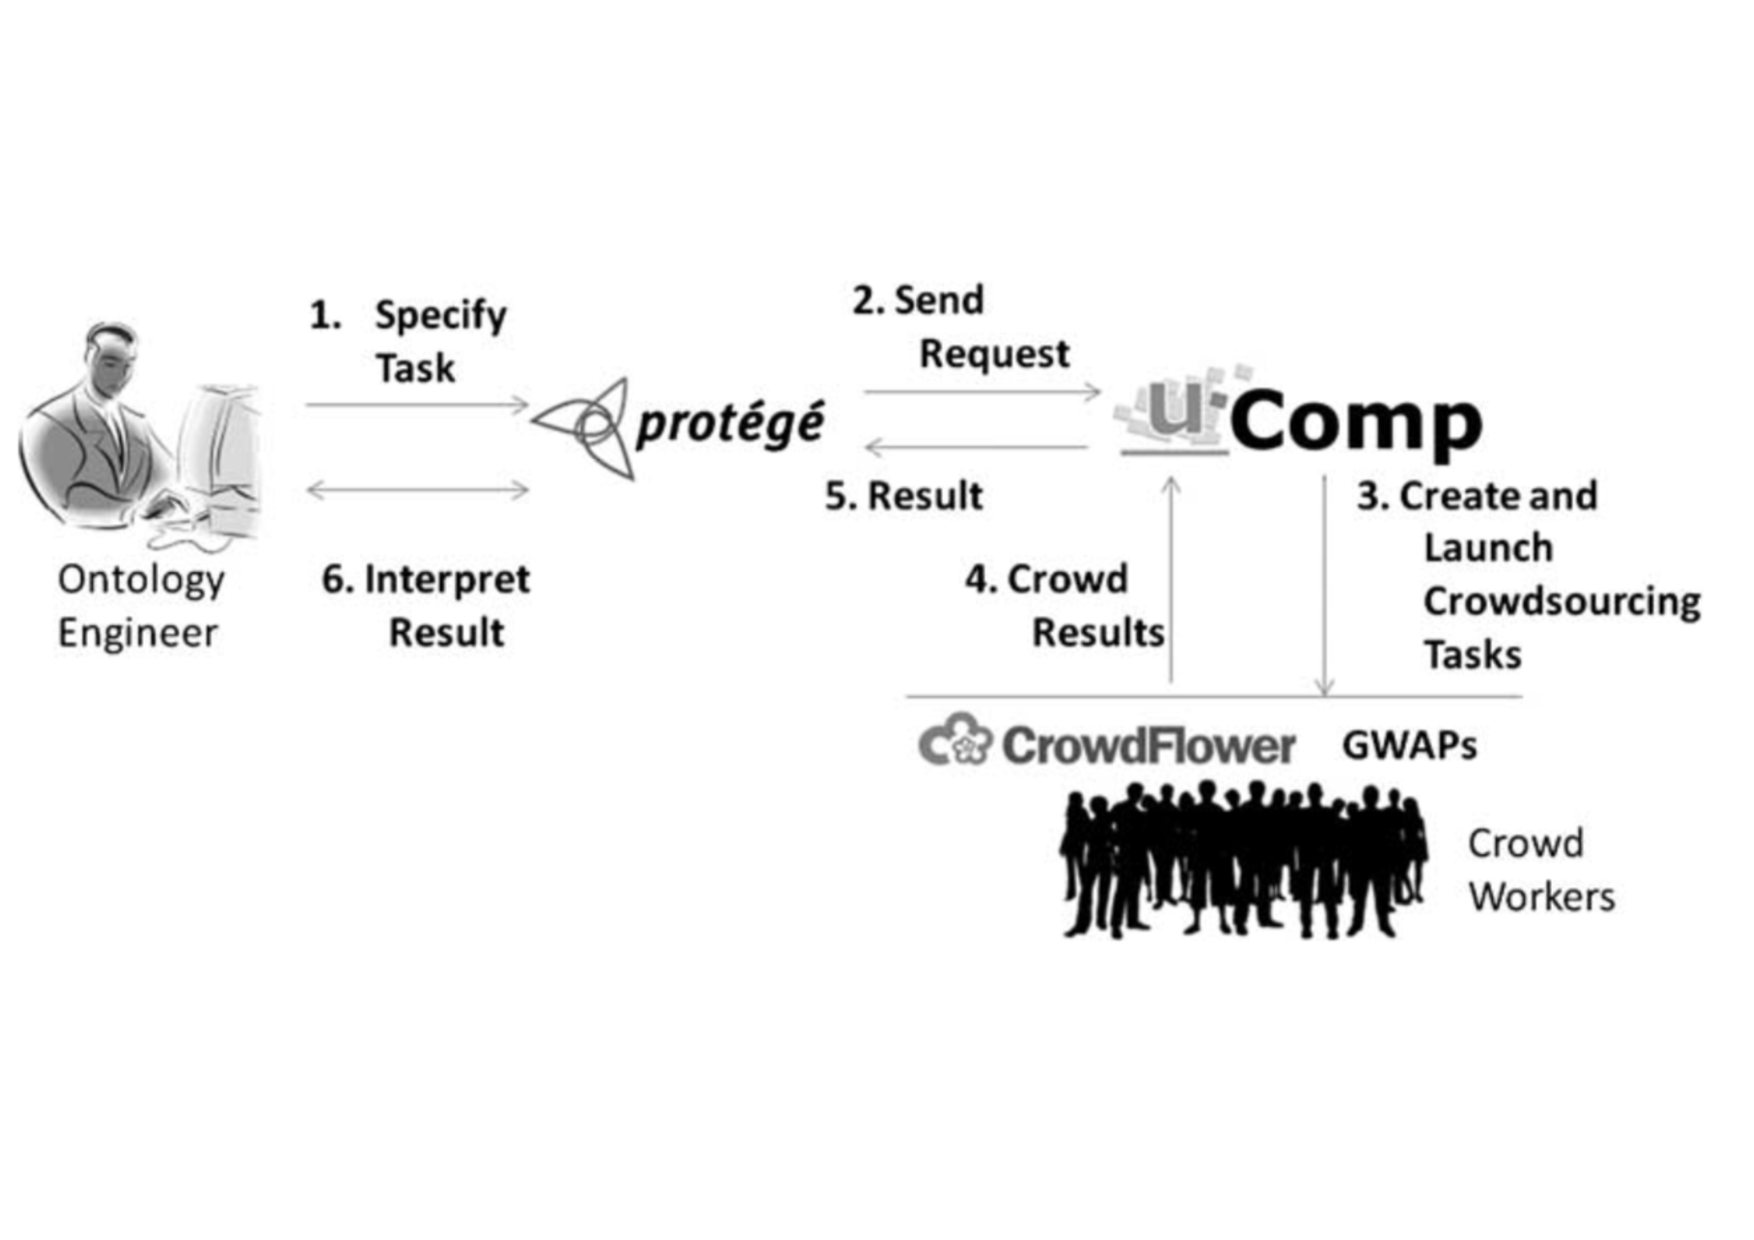
\includegraphics[width=\textwidth]{graphics/ucomp_protege_workflow}
	 \caption{Main workflow to create Crowdsourcing tasks by the uComp Protege Plugin~(adopted from~\cite{wohlgenannt2016})}
	 \label{fig:ucomp_protege_plugin_workflow}
\end{figure}

\begin{enumerate}[label=\textbf{Step \arabic*},leftmargin=\widthof{Step 1}+\labelsep]
	\item \emph{(Task Specification)} In the beginning, the ontology engineer needs to choose from the tasks listed
	in~\hyperref[sec:ucomp_protege_plugin_functionality]{Section~\ref*{sec:ucomp_protege_plugin_functionality}}. For each
	task a standalone interface was created which allows controlling task specific behaviour. 
	\item \emph{(Request Sending)} Next, the plugin gathers the information required to send a request to the uComp platform.
	Unfortunately, at the time of writing this thesis the platform is no longer maintained which required us to directly send the request to the Crowdsourcing provider.  
	\item \emph{(Crowdsourcing Job Creation)} The uComp platform then collects all the data required to create the Crowdsourcing job for the selected Crowdsourcing provider. Initially, the uComp platform supported Crowdflower~(which is now Figure~Eight\footnote{\url{https://www.figure-eight.com/} accessed 2018/07/16}) as the only Crowdsourcing provider. However, the creators of the uComp platform added the option to support other providers as well. 
	\item \emph{(Fetching Crowdsourcing Results)} After job completion~(possibly lasting for several days), the results from the selected Crowdsourcing provider were collected.
	\item \emph{(Aggregating Crowdsourcing Results)} The uComp platform collects all the results~(possibly originating from different platforms) and 
	then calculates the combined result.
	\item \emph{(Result Interpretation)} The last step in the validation workflow is presenting the results to the ontology engineer. Depending on the chosen validation task, further actions may be taken. For example, in case the majority declined the relevance of a specific concept, the ontology engineer may decide to delete the corresponding concept. For all ontology manipulations, the plugin requires manual intervention.
	One of the design goals of the plugin was the guide ontology engineers in doing specific maintenance tasks rather than replacing them by performing these actions automatically. 
\end{enumerate}
